\subsection*{In simulation, estimator selection `recognizes' the covariance structure}
\begin{figure}[htp]
\centering
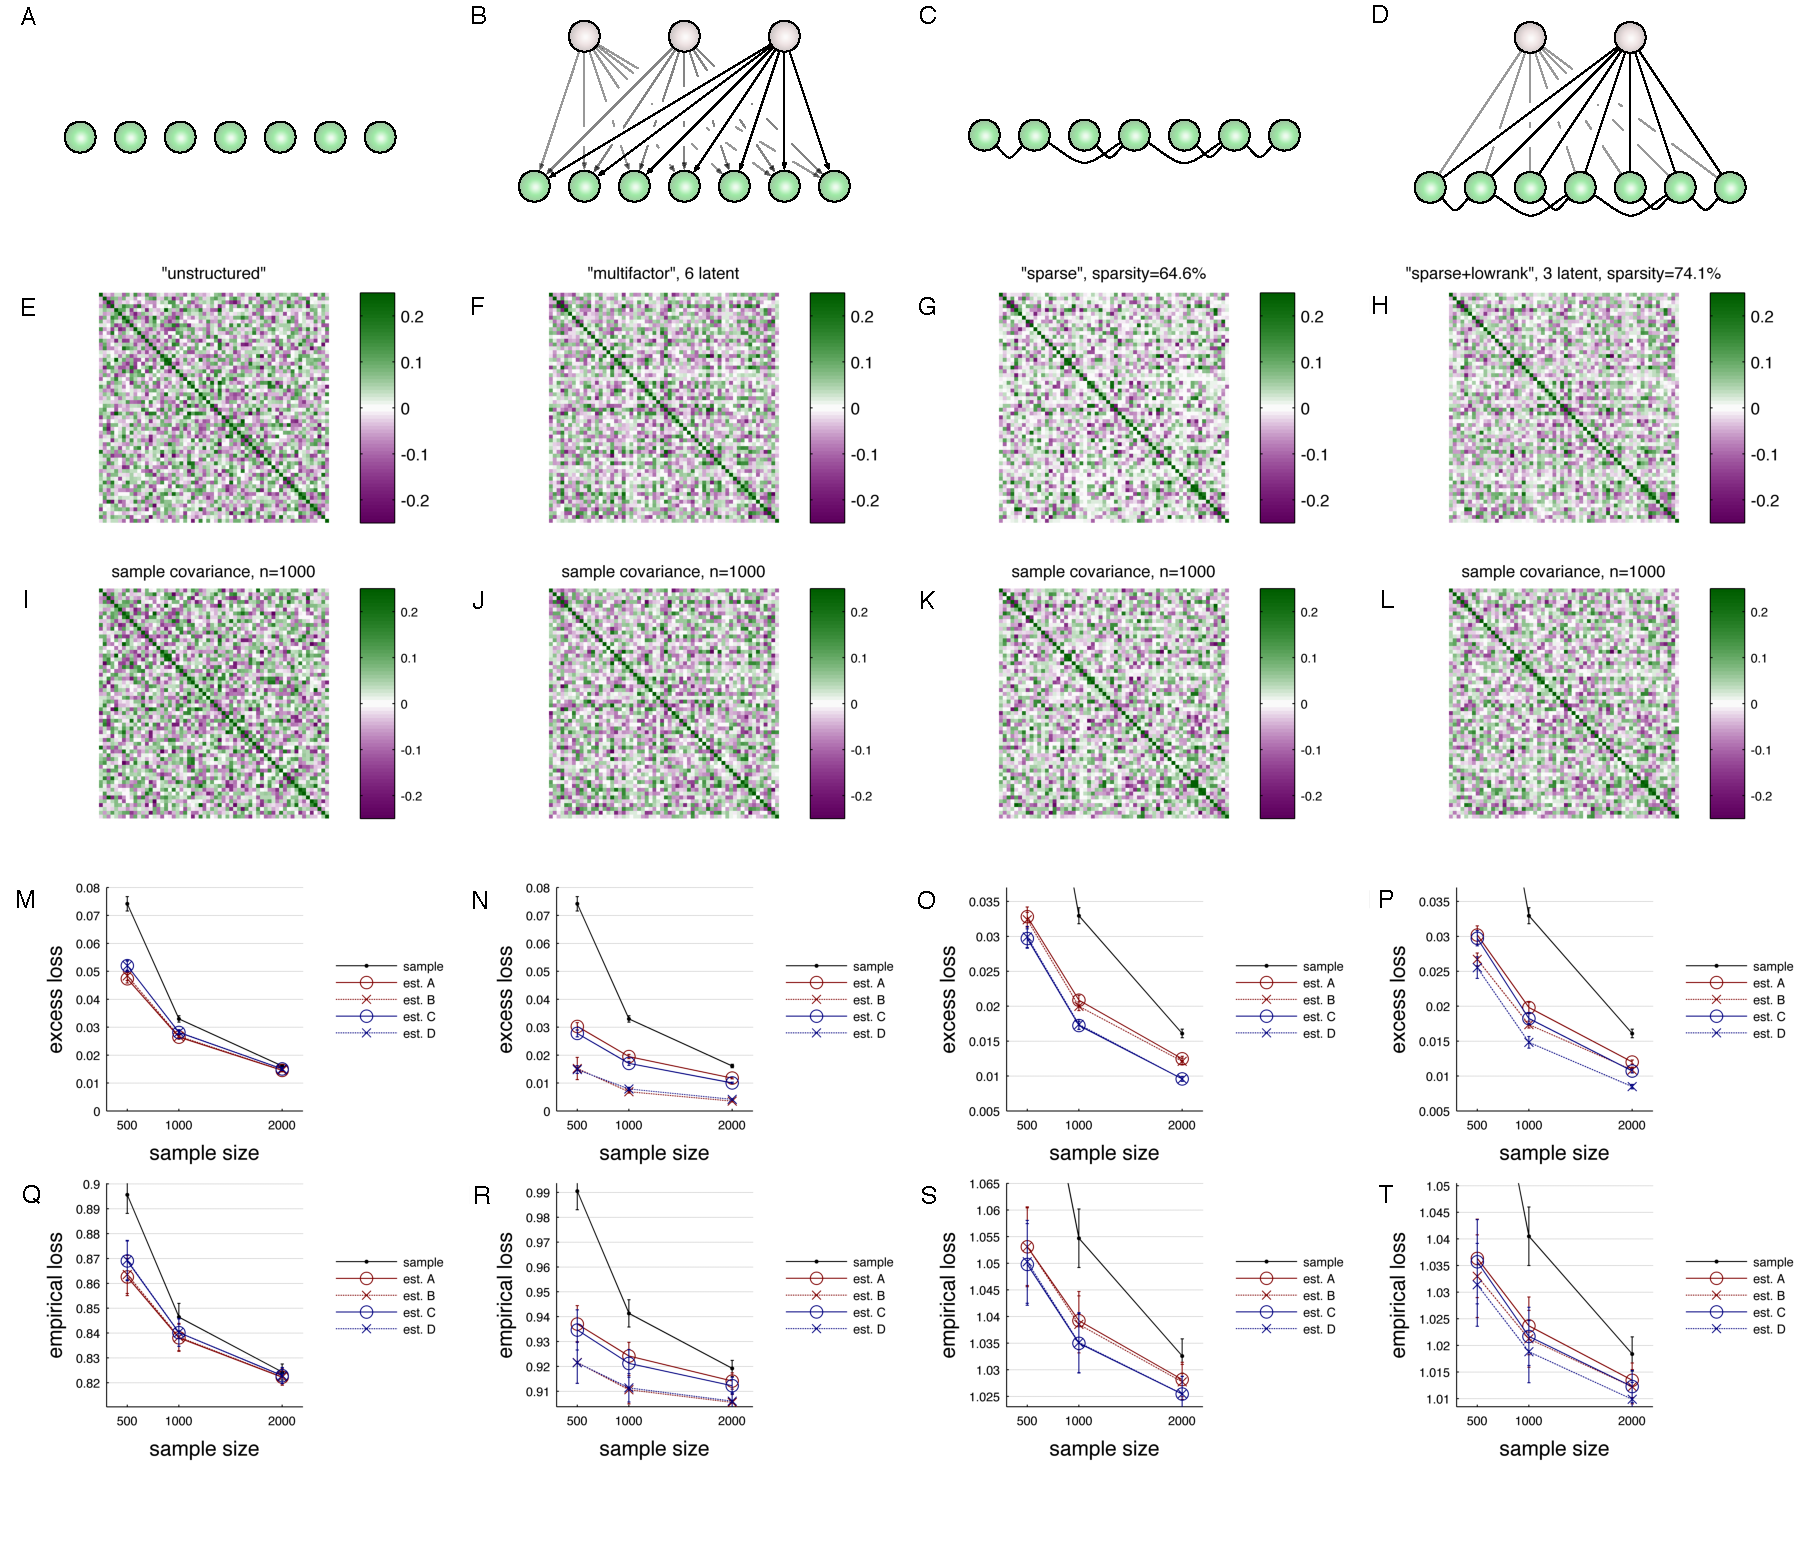
\includegraphics[width=1.0\textwidth]{figures/Figure3.pdf}
\caption{
Selection amongst estimators recognizes covariance atructure.
}\label{fig:03}
\end{figure}


Sample covariance matrices such as E,F,G,H are computed from samples of 1000 independent observations from multivariate normal distributions with true covariance matrices in A,B,C,D, respectively.  However, the true covariance matrices have various low-dimensional structures. 

True matrix A has no low-dimensional structure.  It is computed as the sample covariance matrix of a finite sample (n=1000) of a multivariate Gaussian with independent identically distributed nodes.  

True matrix B is computed by factor analysis of true matrix A with six factors.  

True matrix C is computed by reducing to zero a large fraction the coefficients of the inverse of true matrix A. 

True matrix D is computed by representing the inverse of true matrix A as the sum of a sparse component and a low-low rank component. 

When we estimate the true covariance matrix from the samples of various sizes, we find that for true covariance matrices that have a low-dimensional structure, the covariance estimator whose target has the same type of low-dimensional structure attains lower loss. Plots I,J,K,L show the excess loss, which equals zero when the estimate equals truth (requires knowledge of truth). Plots M,N,O,P show empirical loss computed by cross-validation.  Empirical loss does not require knowledge of truth but is also shifted so that its absolute value is not particularity meaningful but it can be used for comparison. The error bars in these plots indicate the standard deviation, not standard error.

The loss function here is the multivariate log likelihood just as used in the previous post on real data. 

The fact that estimate D outperformed the other estimates can be interpreted that the low-dimensional structure of the covariance matrices obtained from dense microcircuits in the visual cortex is best represented by the sparse+low-rank inverse model. 

We can be then justified to examine the optimal fitted model rather than the sample covariance model in the analysis of neural correlations.  The sparse component represents the graph of interactions in the model, which we can now relate to the circuit architecture.  The low-rank component can be interpreted as common input into the circuit whose properties can be studied separately.

In this way, the process of selecting the best of several regularized covariance estimators serves as the method for recognizing the low-dimensional structure of covariance matrices in a specific domain. 

Note that estimator D performs well on both purely sparse and purely low-rank models. But it does not do better.  Only when the truth is sparse+lowrank does it outperform the other estimates.
